\chapter{User/Item ratings and framing the problem}
\label{ch:user-item}

\section{The user-item matrix}

It's extremely common to hear those who work on Recommendation Systems, talk about matrices, and in particular the user-item matrix. While linear algebra is deep, both mathematically and as it applies to RecSys, we actually will begin with very simplistic relationships. 

Before we get to the matrix forms, let's write down some binary relationships between a set of users and a set of items. For the sake of this example, think of a group of 5 friends (mysteriously named 'A', 'B', 'C', 'D', 'E') and a blind cheese tasting where they're trying out four different cheeses, 'W', 'X', 'Y', 'Z', . The friends are asked to rate the cheeses, 1-5:
\begin{itemize}
    \item \colorbox{yellow}{\parbox{\textwidth-10pt}{
 A starts,  "Ok, I really enjoy W, give that a 5, X \& Y are yummy too, 4, and Z is awful, 1."
}}
    \item \colorbox{yellow}{\parbox{\textwidth-10pt}{
 B replies, "what?! Z is my favorite! 4.5! X \& Y are fine, 3, and W is just ok, 2."
}}
    \item \colorbox{yellow}{\parbox{\textwidth-10pt}{
 B replies, "what?! Z is my favorite! 4.5! X \& Y are fine, 3, and W is just ok, 2."
}}
    \item \colorbox{yellow}{\parbox{\textwidth-10pt}{
 D gives 4,4,5, but we run out of Z before D can try it. 
}}
    \item \colorbox{yellow}{\parbox{\textwidth-10pt}{
 E starts to feel not well, and only tries "W" giving it a 3.
}}
\end{itemize}

The first thing you may notice is that this is a bit annoying to read and parse out. Almost immediately you may want to write this in a more compact and convenient form. Like a collection of lists:

\begin{center}
\begin{math}
\begin{array}{cc}
    A:[5,4,4,1] \\
    B:[2,3,3,4.5] \\
    C:[3,2,3,4] \\
    D:[4,4,5,-] \\
    E:[3,-,-,-] \\
\end{array}
\end{math}
\end{center}
This is relatively ok, but you might want to more clearly indicate the positional meaning in each list:

\begin{lstlisting}[language=Python]
_ = np.nan
scores = np.array([[5,4,4,1],
    [2,3,3,4.5],
    [3,2,3,4],
    [4,4,5,_],
    [3,_,_,_]])
sns.heatmap(
    scores, 
    annot=True, 
    fmt=".1f", 
    xticklabels=['W','X','Y','Z',], 
    yticklabels=['A','B','C','D','E',]
)
\end{lstlisting}

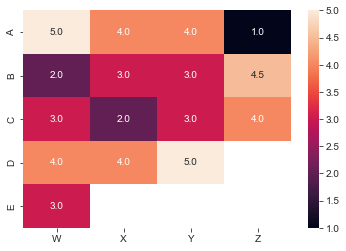
\includegraphics[width=\textwidth-20pt]{book-text/ratings_heatmap.png}

A few natural questions emerge:

\begin{enumerate}
\item What's the most popular cheese? From the observations so far, it's looking like Y is potentially the favorite, but E didn't try Y. 
\item Would D like cheese Z? It seems to be a contentious cheese.
\item If we were asked to buy two cheeses only, which should we buy to satisfy everyone the most?
\end{enumerate}

... and so on. This is cartoonish, and small, but I think the point is clear that this matrix representation above is at least convenient for capturing these ratings.

What may not come obviously is that beyond the convenience of this data visualization, is the mathematical utility of this representation. Question 2 above posits a question that is inherent in the RecSys problem space: "predict how much a user will like an item they've not seen". This question also may be recognizable as a problem from a linear algebra class: "how can we fill in unknown elements of a matrix from the ones we know". This is what is called \emph{matrix completion.}

Before we dive into the linear algebra, let's consider the purely data science perspective called collaborative filtering ([Goldeberg et al, '92](\url{https://d2l.ai/chapter_references/zreferences.html#goldberg-nichols-oki-ea-1992})). The underlying idea is that those with similar taste, help others to know what they like without them having to try it themselves. The collaboration aspect was originally intended to mean among similar-taste users, and the filtering aspect was originally intended to mean filtering out things people wont like.

\section{User-user vs item-item CF}

There are two ways to think of this collaborative filtering strategy:
\begin{itemize}
    \item Two users with similar taste, will continue to have similar taste
    \item Two items with similar user fans, will continue to be popular with other similar users
\end{itemize}

It may sound like these are identical, but perhaps surprisingly, they appear differently in the mathematical interpretations. At a high level, the difference is deciding which kind of similarity do you wish your recommender to make priority of–user similarity or item similarity.

If you prioritize user similarity, then to provide a recommendation for a user $A$, you find a similar user $B$, and then choose a recommendation from $B$'s list of liked content that $A$ hasn't seen  for $A$. 

If you prioritize item similarity, then to provide a recommendation for a user $A$, you find an item that $A$ liked $X$, then you find an item similar to $X$ that $A$ hasn't seen, $Y$, and recommend it for $A$.

Later we will dive deeper into similarity, but let's quickly link these ideas to our brief discussion above. Similar users are rows of the user-item matrix which are similar as vectors; similar items are columns of the user-item matrix which are similar as vectors.


\vspace{10pt}
\colorbox{yellow}{\parbox{\textwidth}{
 \emph{Vector similarity} will be more precisely define later, for now, consider similarity to be computed by normalizing the vectors, and then taking their cosine similarity.
}}
\vspace{10pt}


\subsection{The Netflix challenge}

In 2006, an online competition was kicked off on the website \url{www.thenetflixprize.com}. This competition, was to see if teams could improve on the performance of the Netflix team's collaborative filtering algorithms on an open sourced dataset from the company. While this is more common today via websites like Kaggle or via conference competitions, it was very exciting for those interested in RecSys.

The competition consisted of several intermediate rounds of what were called Progress Prize, and the final Netflix Prize was awarded in 2009. The data provided was a collection of 2,817,131 triples consisting of \lstinline{(user, movie, date_rated)}. And half of these additionally include the rating itself. Notice that like our above example, the user-item information is nearly enough to specify the problem. In this particular dataset, the date was provided. Later on, we will dig into how time might be a factor, and in particular, sequential recommendation systems. 

The stakes were quite high in this competition, requirements for beating the internal performance were a 10\% increase in RMSE (we will discuss this loss function later), but the spoils added up to over \$1.1M. The final winners were BellKor's Pragmatic Chaos(who incidentally one the two previous Progress prizes) with a test RMSE of $0.8567$. In the end, only a $20$-min earlier submission kept BellKor ahead of the competitors The Ensemble. 

c.f. 
\begin{itemize}
\item \url{https://www.researchgate.net/publication/223460749_The_BigChaos_Solution_to_the_Netflix_Grand_Prize}

\item \url{https://www2.seas.gwu.edu/~simhaweb/champalg/cf/papers/ProgressPrize2008_BigChaos.pdf}
\end{itemize}
There are a number of important lessons to be learned from this game, but for the sake of brevity:

\begin{itemize}
\item the user-item matrix is at the heart of collaborative filtering and more generally specifying RecSys problems
\item parameter tuning provided a huge improvement in several algorithms
\item several model innovations came from thinking very hard about the business use-case and human behavior
\item linear algebraic approaches served not only as the first reasonably performant solutions, but building on top of them led to the ultimately winning approach
\item eking out the performance that Netflix originally demanded to win the competition too so long, that business circumstances changed, and the [solution was no longer useful]\url{https://thenextweb.com/news/remember-netflixs-1m-algorithm-contest-well-heres-why-it-didnt-use-the-winning-entry}.
\end{itemize}

That last one might be the \lstinline{most} important thing a machine learning developer needs to learn about recommendations systems: build a working usable model quickly and iterate while the business still cares.


\section{Soft ratings}

In our example above, each cheese received either a numerical rating, or was not tried by a guest. These are what are called **hard ratings**–regardless if the cheese is a brie or a chevre; they are explicit, and their absence indicates a lack of interaction between the user and item. In some contexts, we wish to accommodate circumstances wherein a user does interact with an item, and yet no rating is provided.

A common example is a movies app; a user may have watched a movie with the app, but not provided a star rating. This indicates that the item–in this case a movie–has been observed, but we don't have the rating for our algorithms to learn from. However, we can still make use of this implicit data:

\begin{itemize}
\item we can exclude this item from future recommendations
\item we could separately use this data as a separate term in our learner
\item we could assign a default rating value to indicate "interesting enough to watch, not significant enough to rate"
\end{itemize}

It turns out that implicit ratings are very important for training effective recommendation systems, not only because it's common that users don't give hard ratings, but because they provide a different level of signal. Later, when we wish to train multi-level models to predict both click-likelihood and buy-likelihood, these two levels will prove extremely important.

\section{Data collection and user-tracking}

We established above that we learn both from explicit ratings and implicit ratings, so how and where do we get this data? To dive into this, we'll need to start worrying about application code. In many businesses, the data scientists and ML engineers are separate from the engineers, but for recommendation systems, there's a strong need for alignment between the two functions.

\subsection{What to track}

The simplest and most obvious data collection is user-ratings. If users are given the option to provide ratings or even thumbs-up and thumbs-down, that component will need to be built and that data will be stored. These ratings must be stored not only for the opportunity to build recommendations, it's also a bad user experience to rate something and then shortly thereafter the rating doesn't appear if you revisit the page.

Similarly, it's useful to understand a few other key interactions that we will see can improve and expand your RecSys: \lstinline{page loads}, \lstinline{page views}, \lstinline{clicks}, and \lstinline{add-to-bag}.

For these data, let's use a slightly more complicated example, an e-commerce website. Let's take for this example www.bookshop.org. There are many different applications of RecSys on this one page, almost all of which we will return to in time, but for now let's focus on some interactions.

\vspace{10pt}
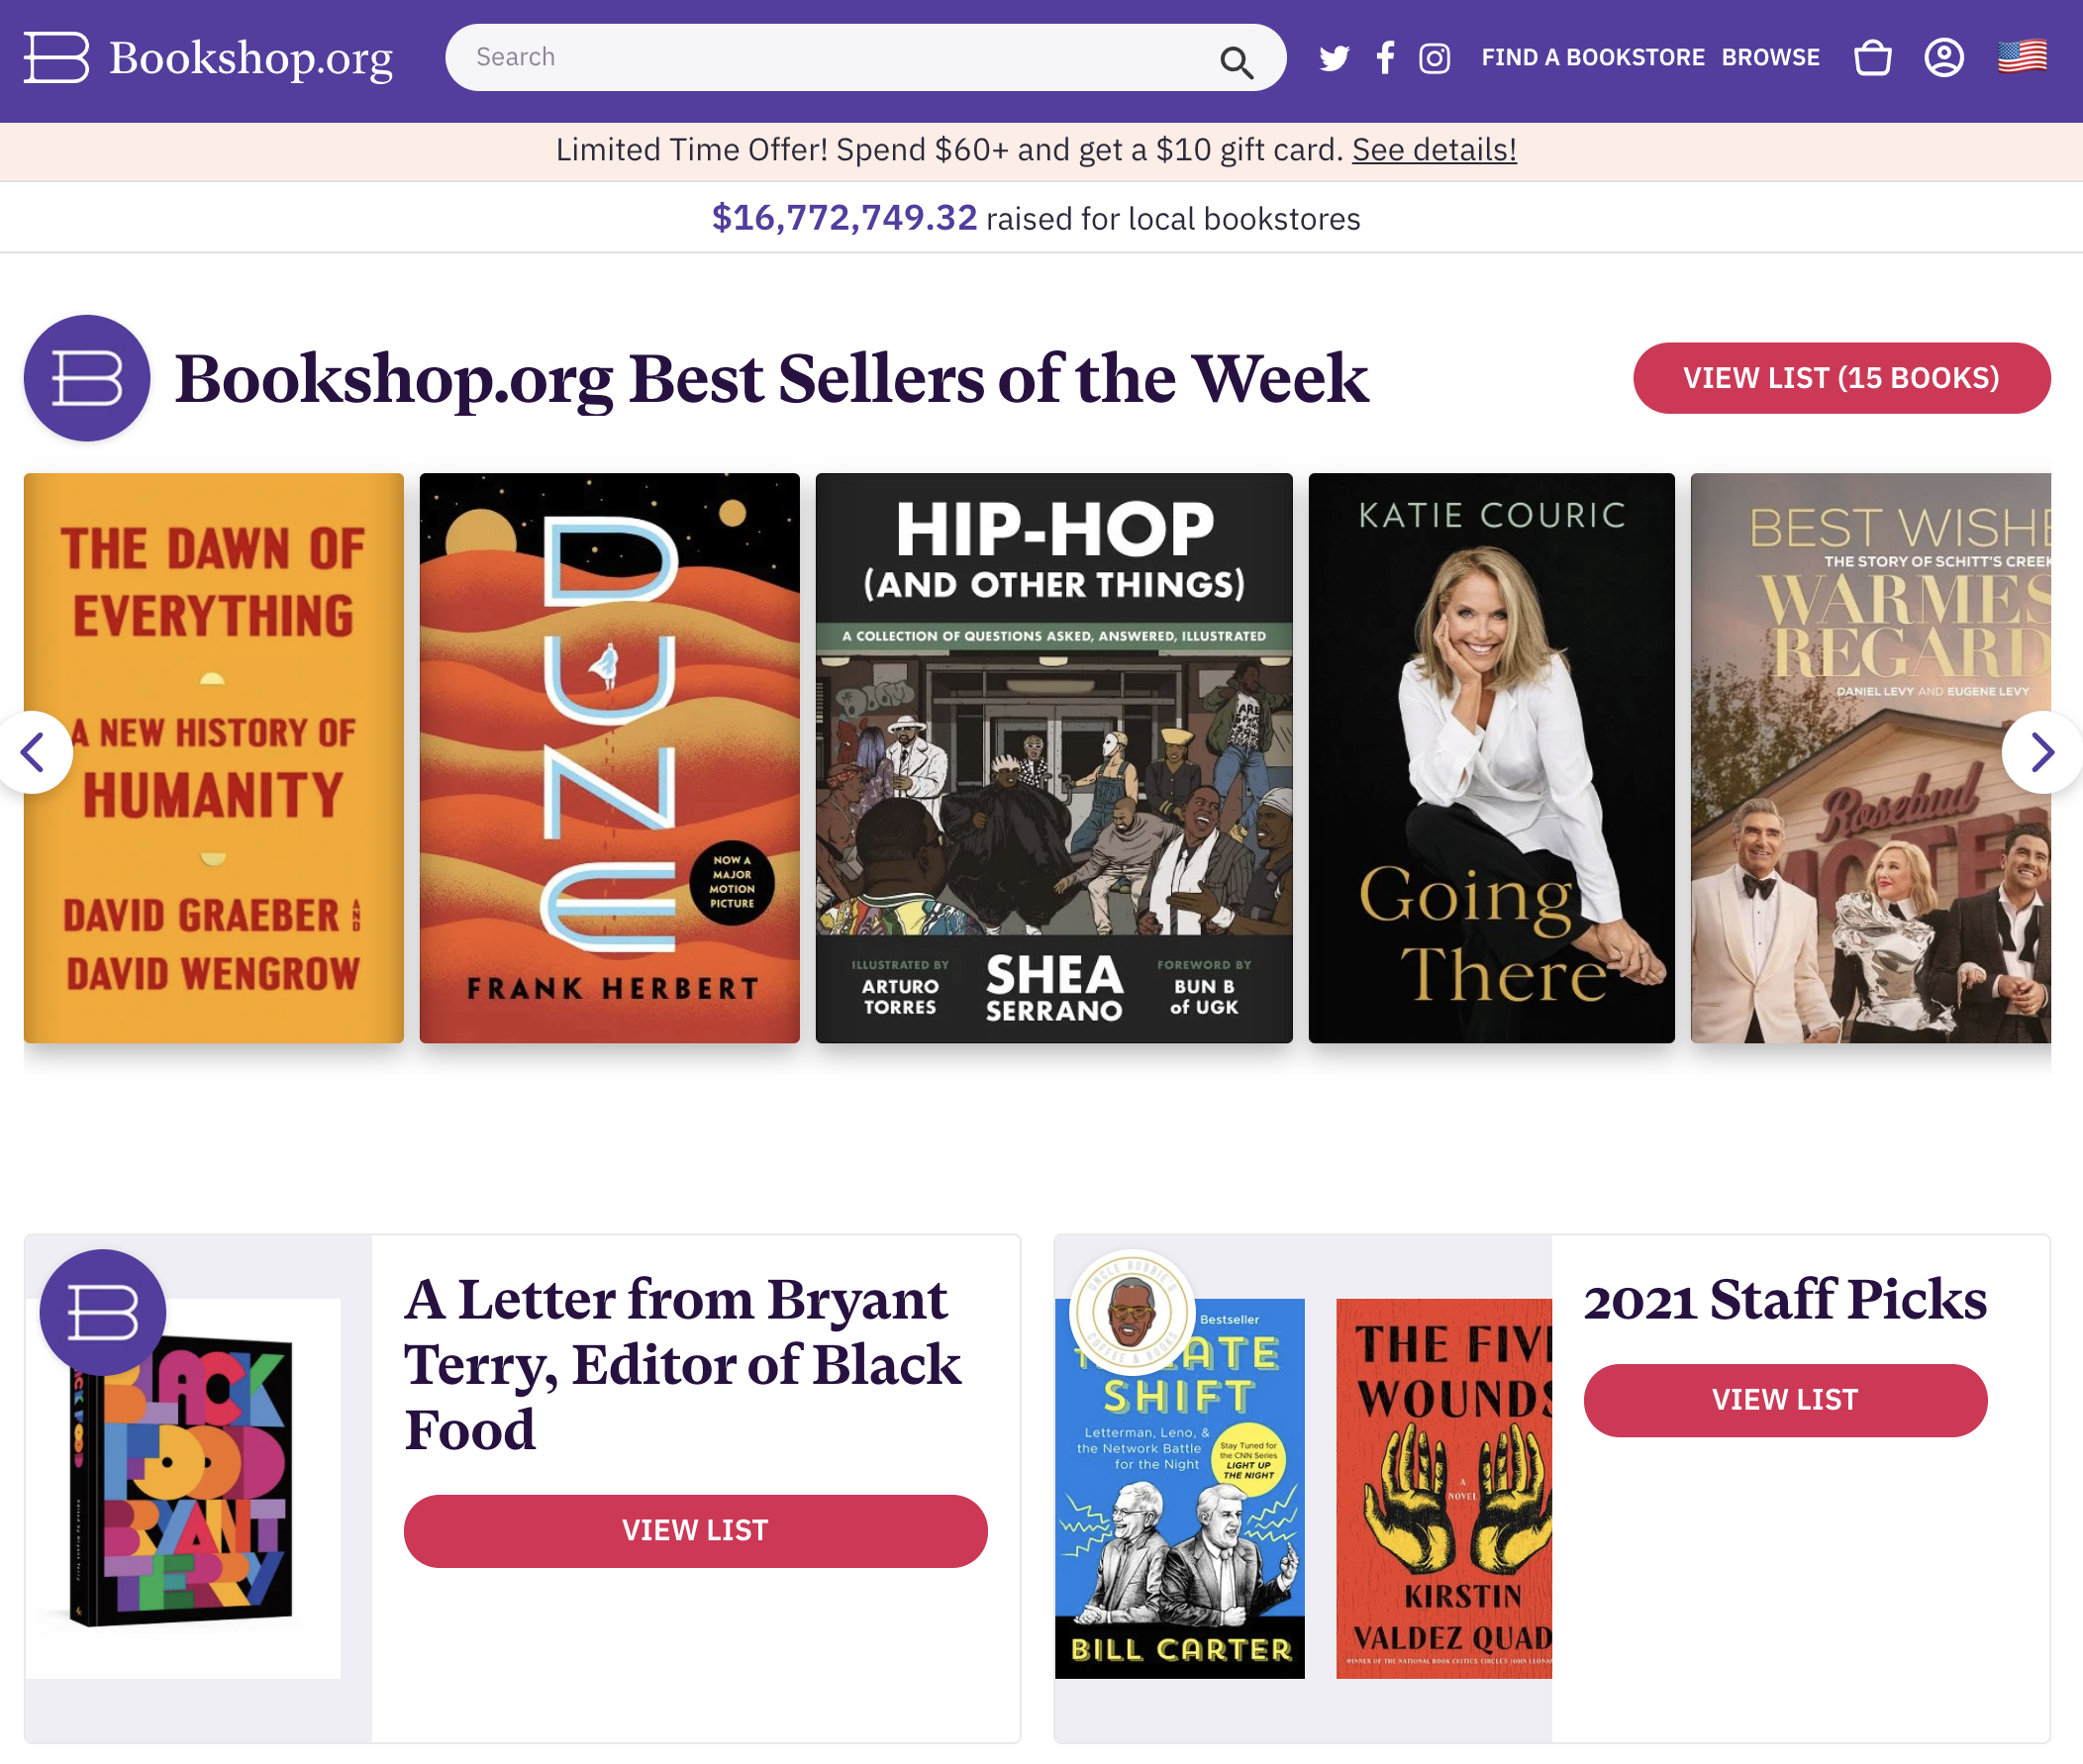
\includegraphics[width=\textwidth-10pt]{book-text/bookshop-landingpage.png}

\paragraph{Page Loads}

When you first load up Bookshop, it starts with items on the page. In the above screenshot, the \emph{Best Sellers of the Week} are all clickable images to those book listings. Despite the user having no choice in this initial page, it's actually quite important to log what is contained in this initial page load. 

These options provide the population of books that the user has seen. If a user has seen an option, then they have the opportunity to click on it, which will ultimately be an important implicit signal. 


\vspace{10pt}
\colorbox{yellow}{\parbox{\textwidth}{ This notion is deeply tied to **propensity score matching;** in mathematics, propensity scores are the probability that an observational unit will be assigned to the treatment vs. the control.
}}
\vspace{10pt}

Compare this to the simple 50-50 A/B test: every unit has a 50\% chance of being exposed to your treatment. In a feature-stratified A/B test, you purposely change the probability of exposure dependent on some feature or collection of features (often called covariates in this context). Those probability of exposures are the propensity scores. 

So why bring up A/B testing here? Later, we'll be interested in mining our soft ratings for signal on user preference, but we must consider the possibility that the lack of a soft rating, is not an implicit bad rating. Thinking back to the cheeses: taster D never had a chance to rate Z, so there's no reason to think D has a preference or aversion in Z. This is because D was not **exposed to Z.** Now thinking back to Bookshop: the page above does not show The Hitchhiker's Guide to the Galaxy, so I have no way to click on it, and thus implicitly communicate that I'm interested in that book. I could use the search, but that's a different kind of signal(which we'll talk about later and, in fact, is a much stronger signal).

When understanding implicit ratings like "did the user look at something" we need to properly account for the entire population of things they were exposed to, and use the inverse of that population size to weight the importance of clicking. For this reason, understanding *all* page loads is important.

\paragraph{Page views and hover}

Websites have gotten much more complicated, and now there are a variety of interactions one must contend with. Look what happens if I click the right arrow in the \emph{Best Sellers of the Week} carousel and then move my mouse over the \emph{Cooking at Home} option:


\vspace{10pt}

\includegraphics[width=\textwidth-10pt]{book-text/bookshop-top-sellers.png}

I've unveiled a new option, and mousing over it, made it larger and have a visual effect. These are ways to communicate to the user more information, and remind the user that these are clickable. To the recommender, these can be used as more implicit feedback.

First, the user clicked the carousel scroll–so some of what they saw in the carousel was interesting enough to dig further. Second, they moused over *Cooking at Home* they might click, or they might just want to see if there's additional information when hovering. Many websites use a hover interaction to provide a pop-up detail. While bookshop doesn't implement something like this; internet users have been trained to expect this behavior by all the websites that do, and so the signal is still meaningful. Third, they've now uncovered a new potential item in their carousel scroll–something we should add to our page loads, but really should come with a higher rating because it required interaction to uncover. 

All this and more can be encoded into the website's logging, rich and verbose logging is one of the most important thing to improve a recommendation system, and it's almost always better to have more than you need rather than the opposite.

\paragraph{Clicks}

If you thought hovering meant interest, wait until you hear about clicking! Not in all cases, but in the large majority, clicking is a very strong indicator of product interest. For e-commerce, clicking often is computed as part of the recommendation team's core KPIs (key performance indicators). 

This is for two reasons:

\begin{itemize}
\item clicking is almost always required to purchase; so it's an upstream filter for all business transactions
\item clicking requires explicit user action; so it's a good measure of intent
\end{itemize}

There will always be noise of course, but clicks are the go-to indicator of what a client is interested in. Many production recommendation systems are trained on click data–not ratings data–because of the much higher data volume and because of strong correlation between click behavior and purchase behavior. 


\vspace{10pt}
\colorbox{yellow}{\parbox{\textwidth}{ Sometimes in Recommendation Systems you hear people talk about 'click-stream' data. It is an important view into clicks data, that also considers the order of a users click in a single 'session'. Modern recommendation systems put a lot of effort into utilizing the order of items a user clicks on, calling this sequential recommendations, and have show dramatic improvements via this additional dimension. We will discuss sequence-based recs later in the book.
}}
\vspace{10pt}

\paragraph{Add to bag}

We've finally arrived, the user has added some item to their bag or cart or queue. This is an extremely strong indicator of interest, and is often very strongly correlated with purchasing. There are even reasons to argue that add-to-bag is a better signal than purchase/order/watch. Add-to-bag is essentially the end of the line for soft ratings, and usually beyond this you'd want to start collecting ratings and reviews.


\paragraph{Collection and instrumentation}

Web applications very frequently instrument all of the above via 'events'. If you don't yet know what events are, maybe ask a buddy in your engineering org–but we'll give you the skinny. Like logging, events are specially formatted message that the application sends out when a certain block of code is executed. Like in the example of a click, the application needs to make a call to get the next content to show the user. It's common to also "fire an event" at this moment indicating information about the user, what they clicked on, the session id for later reference, the time, and various other useful things. This event can be handled downstream in any number of ways, but there's a increasingly possible pattern of it's path bifurcating to:

\begin{itemize}
\item a log database, like a mysql application database tied to the service
\item an event stream for real-time handling
\end{itemize}

The latter is actually what's interesting to us here. Event streams are often connected up to listeners via technologies like Kafka. This kind of infrastructure can get complicated fast (consult your local data engineer or devOps person), but a simple model for what happens is that all of a particular kind of log are sent to a bunch of different destinations that you think can make use of these events.

In the recommender case, an event stream can be connected up to some transformations to process the data for downstream learning tasks. This will be enormously useful if you want to build a recommendation system that uses those logs. Other important uses are real-time metrics tracking for what's going on at any given time on the website.

\subsection{Aside: Funnels}

We've just worked through our first example of a funnel, and no good Data Scientist can avoid thinking about funnels at some point. Like them or hate them, funnel analyses are crucial for critical analyses of your website, and by extension your recommendation system.


\vspace{10pt}
\colorbox{yellow}{\parbox{\textwidth-20pt}{ A \emph{funnel} is a collection of steps a user must take to get from one state to another; it's called a funnel because at each of the discrete steps, a user may stop proceeding through or 'drop off', thus reducing the population size at each step.
}}

\vspace{10pt}
In our discussion of events and user tracking; each step was relevant for a subset of the previous. This means that the process was a funnel, and understanding the drop-off rate at each step, reveals important characteristics of your website, and your recommendations.

\vspace{10pt}
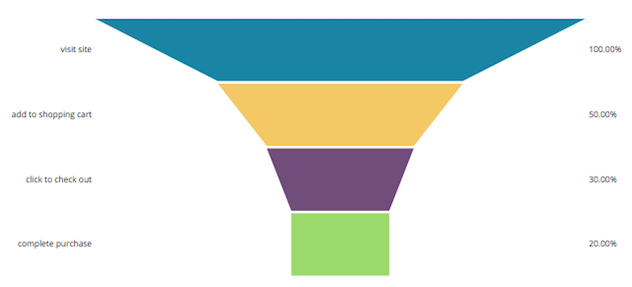
\includegraphics[width=\textwidth-10pt]{book-text/funnel.png}

There are actually three important funnel analyses to be done above:

\begin{itemize}
\item page view to add-to-bag user flow
\item page view to add-to-bag per recommendation
\item add-to-bag to complete purchase
\end{itemize}

The first funnel is merely understanding at a high level, what percentage of users take each step in the above flow. This is a high level measure of your website optimization, the general interestingness of your product offering, and the quality of your user leads.

The second funnel is more fine-grained to take into consideration the recommendations themselves. As mentioned above in the propensity scoring, users can only proceed through the funnel for a particular item if they're shown the item. This intersects with these ideas of funnels because you want to understand at a high level how certain recommendations correlate with funnel drop-off, but also when using a recommender system, the confidence in your recommendations should correlate well with the funnel metrics. We will return to this more in detail later when we discuss loss functions, but for now you should remember to think of different categories of recommendation-user pairs and how their funnels may look compared to average.

Finally, add-to-bag to completion. This actually isn't part of the RecSys problem, but should be on your mind as a Data Scientist or Machine Learning engineer trying to improve the product. **No matter how good your recommendations are, this funnel may destroy any of your hard work.** Before working on a recommender problem, you should almost always investigate the funnel performance in getting a user from add-to-bag to check-out-completed. If there's something cumbersome, or difficult about this flow, it will almost certainly provide a bigger bang-for-your-buck to fix this, than to improve recommendations. Investigate the drop-offs, do user-studies to understand what might be confusing, work with product and engineering to ensure everyone is aligned on this flow before you start building a recommender for e-commerce.

\section{Business insight and what people like}

In the above example from Bookshop.org, we notice that *Top Sellers of the Week* is the primary carousel on the page. Recall our earlier work on \lstinline{get_most_popular_recs}, this is simply that recommender but applied to a specific Collector–one that only looks in the last week. 

This carousel is an example of a recommender providing business-insight, in addition to driving recommendations. A common mission of a growth team is to understand weekly trends and KPIs, often things like weekly-active-users, and new signups. For many digital-first companies, growth teams are additionally interested in understanding the primary drivers.

Let's take an example: as of the writing of this, the Netflix show ***Squid Game*** became Netflix' most popular series of all time, breaking a huge number of records in the process. Squid Game achieved 111 Million viewers in the first month. Most obviously, *Squid Game* needs to be featured in *Top Shows of the Week* or *Hottest Titles* carousels, but what else does a breakout hit like this matter?

The first important insight companies almost always ask for is **attribution**–if the numbers go up in a week, what led to that? Is there something important or special about launches that drove additional growth? How can we learn from that to do better in the future? In the case of *Squid Game*–a foreign-language show that saw massive interest with an English-speaking crowd–executives might take away the inclination to invest more in shows from South Korea, or subtitled shows with high-drama. The flip side of this coin is also important, when growth metrics lag, executives nearly always ask why–being able to point to what was the most popular, and how it may have deviated from expectation, helps a lot.

The other important insight can feed back into recommendations; during exciting debuts like *Squid Game*, it's easy to get caught up in the excitement as you see all your metrics go up and to the right, but might this negatively effect things also? If you have a debut show the same week or two as *Squid Game's* you'll be less enthusiastic about all this success. Overall, successes like this usually drive *incremental* growth which is great for business, and in total, metrics will all probably look up. Other items however may have less successful launches due to a zero-sum game amongst the core user base. This can have a negative effect on longer term metrics, and even can make later recommendations less effective. 

Later, we will learn about diversity of recommendations. There are a large number of reasons to care about diversifying your recommendations, but here we observe one which is to increase the overall matching valence of your users with items. As you keep a broad base of users highly engaged, you increase your future opportunity for growth.

\vspace{10pt}
\colorbox{yellow}{\parbox{\textwidth-20pt}{ \emph{Incremental gains} is a term modified from economics and put to use in growth marketing and growth analytics. Incremental gains refer to a margin of increase in addition to the gains expected from an expended effort. A simple example would be a business that usually adds a user for ever \$100 in marketing spend, gets some positive press, and the next week they get a user for every \$80 in marketing spend. If they keep their marketing budget fixed that week at \$1600, they would get 20 new users instead of 16; an incremental gain of 4 users. This is especially common when testing new treatments or programs.
}}

\vspace{10pt}
Finally, beyond surfacing the trending hits, another benefit of knowing what's really hot on your platform or service, is advertising. When a phenomenon starts, there can be a huge advantage in priming the pump, i.e. making noise and publicity of the success. This sometimes leads to a network effect, and in the days with viral content and easy distribution, this can have multiplier effects on your platform's growth.